\section{Objective and Sub-Tasks}
\label{sec:objective}
The main objective of this work is the development of a radar-based odometry system that estimates vehicle ego-motion using a single mmWave radar sensor.  
The motivation behind this approach is to explore radar as a cost-efficient and robust alternative to vision- or LiDAR-based odometry, particularly under adverse weather and lighting conditions.  
The system is designed to process radar point clouds in real time, extract motion information, and generate reliable pose estimates that can be used for autonomous navigation and digital twin construction.  

\begin{figure}[!htbp]
    \centering
    %\resizebox{0.48\textwidth}{!}{
        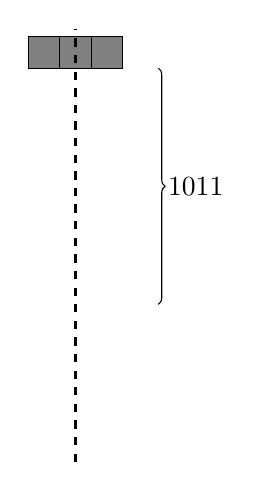
\begin{tikzpicture}
            \gokart{0}{0}{0}
        
            %Wall (three cubes)
            \draw[fill=gray] (-0.6,3) rectangle (-0.2,3.4);
            \draw[fill=gray] (-0.2,3) rectangle (0.2,3.4);
            \draw[fill=gray] (0.2,3) rectangle (0.6,3.4);
        
            %Dashed line from go-kart to wall
            \draw[dashed, thick] (0,-2) -- (0,3.5);

            \draw [decorate, decoration = {brace, raise=10pt}] (0.7,3) -- (0.7, 0) node[pos=0.5,right=10pt,black]{\SIrange{10}{11}{\meter}};
        \end{tikzpicture}
    %}
    \caption{Test scenario}
    \label{fig:test_scenario}
\end{figure}
The experimental setup consists of a Texas Instruments IWR6843AOPEVM development board, featuring the IWR6843AOP mmWave radar sensor, mounted at the front of a vehicle.  
The sensor provides point cloud data enriched with range, angle, and Doppler velocity information.  
This data forms the basis for the processing pipeline and enables the evaluation of radar odometry performance under realistic driving scenarios.  


\subsection{Sub-Tasks}

The research objective, together with the constraints of using a single radar sensor, implied several practical sub-tasks:  
\begin{itemize}
    \item Designing a pipeline to acquire and decode raw radar data.  
    \item Investigating suitable sensor configurations to balance field of view, update rate, and data density.  
    \item Implementing clustering methods to structure radar detections and isolate relevant features.  
    \item Integrating Doppler velocity information into the odometry estimation process.  
    \item Developing scan-to-scan registration using iterative closest point (ICP) optimization.  
    \item Employing submap aggregation to mitigate sparsity and improve stability.  
    \item Incorporating cluster-based tracking to filter dynamic objects from the ego-motion estimation.  
    \item Validating the complete system using recorded datasets and controlled driving experiments.  
\end{itemize}

As each sub-task builds upon the results of the previous one, the work followed an iterative and modular development approach, enabling gradual integration and continuous evaluation of the proposed system.  